\documentclass[twoside]{book}

% Packages required by doxygen
\usepackage{fixltx2e}
\usepackage{calc}
\usepackage{doxygen}
\usepackage[export]{adjustbox} % also loads graphicx
\usepackage{graphicx}
\usepackage[utf8]{inputenc}
\usepackage{makeidx}
\usepackage{multicol}
\usepackage{multirow}
\PassOptionsToPackage{warn}{textcomp}
\usepackage{textcomp}
\usepackage[nointegrals]{wasysym}
\usepackage[table]{xcolor}

% Font selection
\usepackage[T1]{fontenc}
\usepackage[scaled=.90]{helvet}
\usepackage{courier}
\usepackage{amssymb}
\usepackage{sectsty}
\renewcommand{\familydefault}{\sfdefault}
\allsectionsfont{%
  \fontseries{bc}\selectfont%
  \color{darkgray}%
}
\renewcommand{\DoxyLabelFont}{%
  \fontseries{bc}\selectfont%
  \color{darkgray}%
}
\newcommand{\+}{\discretionary{\mbox{\scriptsize$\hookleftarrow$}}{}{}}

% Page & text layout
\usepackage{geometry}
\geometry{%
  a4paper,%
  top=2.5cm,%
  bottom=2.5cm,%
  left=2.5cm,%
  right=2.5cm%
}
\tolerance=750
\hfuzz=15pt
\hbadness=750
\setlength{\emergencystretch}{15pt}
\setlength{\parindent}{0cm}
\setlength{\parskip}{3ex plus 2ex minus 2ex}
\makeatletter
\renewcommand{\paragraph}{%
  \@startsection{paragraph}{4}{0ex}{-1.0ex}{1.0ex}{%
    \normalfont\normalsize\bfseries\SS@parafont%
  }%
}
\renewcommand{\subparagraph}{%
  \@startsection{subparagraph}{5}{0ex}{-1.0ex}{1.0ex}{%
    \normalfont\normalsize\bfseries\SS@subparafont%
  }%
}
\makeatother

% Headers & footers
\usepackage{fancyhdr}
\pagestyle{fancyplain}
\fancyhead[LE]{\fancyplain{}{\bfseries\thepage}}
\fancyhead[CE]{\fancyplain{}{}}
\fancyhead[RE]{\fancyplain{}{\bfseries\leftmark}}
\fancyhead[LO]{\fancyplain{}{\bfseries\rightmark}}
\fancyhead[CO]{\fancyplain{}{}}
\fancyhead[RO]{\fancyplain{}{\bfseries\thepage}}
\fancyfoot[LE]{\fancyplain{}{}}
\fancyfoot[CE]{\fancyplain{}{}}
\fancyfoot[RE]{\fancyplain{}{\bfseries\scriptsize Generated by Doxygen }}
\fancyfoot[LO]{\fancyplain{}{\bfseries\scriptsize Generated by Doxygen }}
\fancyfoot[CO]{\fancyplain{}{}}
\fancyfoot[RO]{\fancyplain{}{}}
\renewcommand{\footrulewidth}{0.4pt}
\renewcommand{\chaptermark}[1]{%
  \markboth{#1}{}%
}
\renewcommand{\sectionmark}[1]{%
  \markright{\thesection\ #1}%
}

% Indices & bibliography
\usepackage{natbib}
\usepackage[titles]{tocloft}
\setcounter{tocdepth}{3}
\setcounter{secnumdepth}{5}
\makeindex

% Hyperlinks (required, but should be loaded last)
\usepackage{ifpdf}
\ifpdf
  \usepackage[pdftex,pagebackref=true]{hyperref}
\else
  \usepackage[ps2pdf,pagebackref=true]{hyperref}
\fi
\hypersetup{%
  colorlinks=true,%
  linkcolor=blue,%
  citecolor=blue,%
  unicode%
}

% Custom commands
\newcommand{\clearemptydoublepage}{%
  \newpage{\pagestyle{empty}\cleardoublepage}%
}

\usepackage{caption}
\captionsetup{labelsep=space,justification=centering,font={bf},singlelinecheck=off,skip=4pt,position=top}

%===== C O N T E N T S =====

\begin{document}

% Titlepage & ToC
\hypersetup{pageanchor=false,
             bookmarksnumbered=true,
             pdfencoding=unicode
            }
\pagenumbering{roman}
\begin{titlepage}
\vspace*{7cm}
\begin{center}%
{\Large earth\+L\+C\+D-\/\+G\+UI }\\
\vspace*{1cm}
{\large Generated by Doxygen 1.8.11}\\
\end{center}
\end{titlepage}
\clearemptydoublepage
\tableofcontents
\clearemptydoublepage
\pagenumbering{arabic}
\hypersetup{pageanchor=true}

%--- Begin generated contents ---
\chapter{Hierarchical Index}
\section{Class Hierarchy}
This inheritance list is sorted roughly, but not completely, alphabetically\+:\begin{DoxyCompactList}
\item object\begin{DoxyCompactList}
\item \contentsline{section}{ez\+G\+F\+X.\+earth\+L\+C\+D.\+earth\+L\+CD}{\pageref{classez_g_f_x_1_1earth_l_c_d_1_1earth_l_c_d}}{}
\end{DoxyCompactList}
\end{DoxyCompactList}

\chapter{Class Index}
\section{Class List}
Here are the classes, structs, unions and interfaces with brief descriptions\+:\begin{DoxyCompactList}
\item\contentsline{section}{\hyperlink{classez_g_f_x_1_1earth_l_c_d_1_1earth_l_c_d}{ez\+G\+F\+X.\+earth\+L\+C\+D.\+earth\+L\+CD} \\*Class for earth lcd }{\pageref{classez_g_f_x_1_1earth_l_c_d_1_1earth_l_c_d}}{}
\end{DoxyCompactList}

\chapter{Class Documentation}
\hypertarget{classez_g_f_x_1_1earth_l_c_d_1_1earth_l_c_d}{}\section{ez\+G\+F\+X.\+earth\+L\+C\+D.\+earth\+L\+CD Class Reference}
\label{classez_g_f_x_1_1earth_l_c_d_1_1earth_l_c_d}\index{ez\+G\+F\+X.\+earth\+L\+C\+D.\+earth\+L\+CD@{ez\+G\+F\+X.\+earth\+L\+C\+D.\+earth\+L\+CD}}


Class for earth lcd.  


Inheritance diagram for ez\+G\+F\+X.\+earth\+L\+C\+D.\+earth\+L\+CD\+:\begin{figure}[H]
\begin{center}
\leavevmode
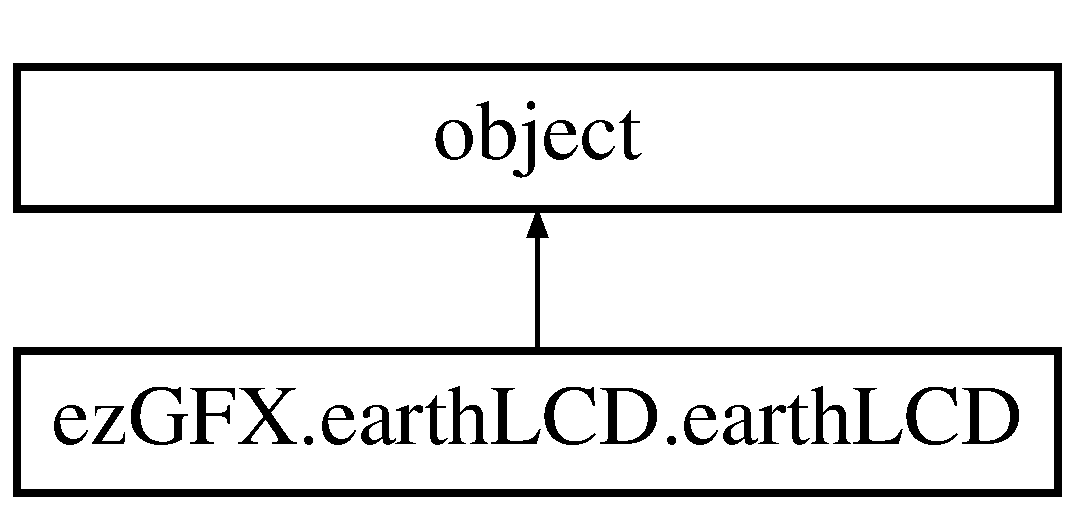
\includegraphics[height=2.000000cm]{classez_g_f_x_1_1earth_l_c_d_1_1earth_l_c_d}
\end{center}
\end{figure}
\subsection*{Public Member Functions}
\begin{DoxyCompactItemize}
\item 
def \hyperlink{classez_g_f_x_1_1earth_l_c_d_1_1earth_l_c_d_a306a9a9eb6568e0be19c6d8ac665bb71}{\+\_\+\+\_\+init\+\_\+\+\_\+} (self, size)
\begin{DoxyCompactList}\small\item\em Constructs the object. \end{DoxyCompactList}\item 
def \hyperlink{classez_g_f_x_1_1earth_l_c_d_1_1earth_l_c_d_acfbcb9fb412431cf0fe4349fd503667a}{clear\+Screen} (self, color)
\begin{DoxyCompactList}\small\item\em \{ function\+\_\+description \} \end{DoxyCompactList}\item 
def \hyperlink{classez_g_f_x_1_1earth_l_c_d_1_1earth_l_c_d_a176dfa3881b7ff05ca1862f01a1461fe}{create\+Background} (self, color, image=None)
\begin{DoxyCompactList}\small\item\em Creates a background. \end{DoxyCompactList}\item 
def \hyperlink{classez_g_f_x_1_1earth_l_c_d_1_1earth_l_c_d_a3ec38493a38bd0678c8bf1375791ce91}{create\+Button} (self, id, location, image\+Up, image\+Down, state, callback)
\begin{DoxyCompactList}\small\item\em Creates a button. \end{DoxyCompactList}\item 
def \hyperlink{classez_g_f_x_1_1earth_l_c_d_1_1earth_l_c_d_a46c991c382ce6d57490d1f9241c748cf}{create\+Checkbox} (self, id, location, checked\+Image, unchecked\+Image, state, callback, text)
\begin{DoxyCompactList}\small\item\em Creates a checkbox. \end{DoxyCompactList}\item 
def \hyperlink{classez_g_f_x_1_1earth_l_c_d_1_1earth_l_c_d_a37b3d546e5bb76e53ff08174b35ec916}{update\+Button} (self, id, state)
\begin{DoxyCompactList}\small\item\em \{ function\+\_\+description \} \end{DoxyCompactList}\item 
def \hyperlink{classez_g_f_x_1_1earth_l_c_d_1_1earth_l_c_d_abb9f7fbcf73964522ed6d7da5ba3b8e2}{update\+Checkbox} (self, id, state)
\begin{DoxyCompactList}\small\item\em \{ function\+\_\+description \} \end{DoxyCompactList}\item 
def \hyperlink{classez_g_f_x_1_1earth_l_c_d_1_1earth_l_c_d_aba453c9d165b50ef8fda463b31d8af74}{create\+Text\+Box} (self, id, location, font, size, text, color, position=\textquotesingle{}Left\textquotesingle{}, style=None, save\+Background=False)
\begin{DoxyCompactList}\small\item\em Creates a text box. \end{DoxyCompactList}\item 
def \hyperlink{classez_g_f_x_1_1earth_l_c_d_1_1earth_l_c_d_a4dd0ce88479753b6b717b6c18ada01c9}{update\+Text\+Box} (self, id, text, color)
\begin{DoxyCompactList}\small\item\em \{ function\+\_\+description \} \end{DoxyCompactList}\item 
def \hyperlink{classez_g_f_x_1_1earth_l_c_d_1_1earth_l_c_d_ae100f4bc0bafaead25d23280110509f6}{check\+Widgets} (self, x, y)
\begin{DoxyCompactList}\small\item\em \{ call with x and y and will return widget id or None \} \end{DoxyCompactList}\end{DoxyCompactItemize}
\subsection*{Static Public Attributes}
\begin{DoxyCompactItemize}
\item 
int {\bfseries button} = 0\hypertarget{classez_g_f_x_1_1earth_l_c_d_1_1earth_l_c_d_a68bf8834823c0e523999362f16703d66}{}\label{classez_g_f_x_1_1earth_l_c_d_1_1earth_l_c_d_a68bf8834823c0e523999362f16703d66}

\item 
int {\bfseries text\+Box} = 1\hypertarget{classez_g_f_x_1_1earth_l_c_d_1_1earth_l_c_d_a641ca6ae11a11fb4f7c10d0e521b11ba}{}\label{classez_g_f_x_1_1earth_l_c_d_1_1earth_l_c_d_a641ca6ae11a11fb4f7c10d0e521b11ba}

\item 
int {\bfseries check\+Box} = 2\hypertarget{classez_g_f_x_1_1earth_l_c_d_1_1earth_l_c_d_ad58211b5ca4480cf5c7007ad52678428}{}\label{classez_g_f_x_1_1earth_l_c_d_1_1earth_l_c_d_ad58211b5ca4480cf5c7007ad52678428}

\item 
int {\bfseries check\+Box\+State\+Un\+Checked} = 0\hypertarget{classez_g_f_x_1_1earth_l_c_d_1_1earth_l_c_d_a13217f0025f0df884653c022dc155686}{}\label{classez_g_f_x_1_1earth_l_c_d_1_1earth_l_c_d_a13217f0025f0df884653c022dc155686}

\item 
int {\bfseries check\+Box\+State\+Checked} = 1\hypertarget{classez_g_f_x_1_1earth_l_c_d_1_1earth_l_c_d_a056a2ee5437c1472d2ff7fdbc05b2860}{}\label{classez_g_f_x_1_1earth_l_c_d_1_1earth_l_c_d_a056a2ee5437c1472d2ff7fdbc05b2860}

\item 
int {\bfseries check\+Box\+State\+Toggle} = 2\hypertarget{classez_g_f_x_1_1earth_l_c_d_1_1earth_l_c_d_a406367c92e3232626f5aa5b8f8a2f711}{}\label{classez_g_f_x_1_1earth_l_c_d_1_1earth_l_c_d_a406367c92e3232626f5aa5b8f8a2f711}

\item 
int {\bfseries check\+Box\+State\+Disabled} = 3\hypertarget{classez_g_f_x_1_1earth_l_c_d_1_1earth_l_c_d_ad7c49dcba9d7753236bcc7ff8ba419d6}{}\label{classez_g_f_x_1_1earth_l_c_d_1_1earth_l_c_d_ad7c49dcba9d7753236bcc7ff8ba419d6}

\item 
int {\bfseries button\+State\+Up} = 0\hypertarget{classez_g_f_x_1_1earth_l_c_d_1_1earth_l_c_d_ad941b7c5339a87a7e588e020190db4a6}{}\label{classez_g_f_x_1_1earth_l_c_d_1_1earth_l_c_d_ad941b7c5339a87a7e588e020190db4a6}

\item 
int {\bfseries button\+State\+Down} = 1\hypertarget{classez_g_f_x_1_1earth_l_c_d_1_1earth_l_c_d_a6b50be2bc5f3e3abc069ed31b55519ef}{}\label{classez_g_f_x_1_1earth_l_c_d_1_1earth_l_c_d_a6b50be2bc5f3e3abc069ed31b55519ef}

\item 
int {\bfseries button\+State\+Disabled} = 2\hypertarget{classez_g_f_x_1_1earth_l_c_d_1_1earth_l_c_d_ab0346623c9ccc9cfa156bff71bcd776a}{}\label{classez_g_f_x_1_1earth_l_c_d_1_1earth_l_c_d_ab0346623c9ccc9cfa156bff71bcd776a}

\item 
{\bfseries screen} = None\hypertarget{classez_g_f_x_1_1earth_l_c_d_1_1earth_l_c_d_a5707e94673b2aa1187f1c038442d2344}{}\label{classez_g_f_x_1_1earth_l_c_d_1_1earth_l_c_d_a5707e94673b2aa1187f1c038442d2344}

\item 
list {\bfseries widgets} = \mbox{[}$\,$\mbox{]}\hypertarget{classez_g_f_x_1_1earth_l_c_d_1_1earth_l_c_d_a2037a56cb78849093e6e5845ad066f4d}{}\label{classez_g_f_x_1_1earth_l_c_d_1_1earth_l_c_d_a2037a56cb78849093e6e5845ad066f4d}

\end{DoxyCompactItemize}


\subsection{Detailed Description}
Class for earth lcd. 

\subsection{Constructor \& Destructor Documentation}
\index{ez\+G\+F\+X\+::earth\+L\+C\+D\+::earth\+L\+CD@{ez\+G\+F\+X\+::earth\+L\+C\+D\+::earth\+L\+CD}!\+\_\+\+\_\+init\+\_\+\+\_\+@{\+\_\+\+\_\+init\+\_\+\+\_\+}}
\index{\+\_\+\+\_\+init\+\_\+\+\_\+@{\+\_\+\+\_\+init\+\_\+\+\_\+}!ez\+G\+F\+X\+::earth\+L\+C\+D\+::earth\+L\+CD@{ez\+G\+F\+X\+::earth\+L\+C\+D\+::earth\+L\+CD}}
\subsubsection[{\texorpdfstring{\+\_\+\+\_\+init\+\_\+\+\_\+(self, size)}{__init__(self, size)}}]{\setlength{\rightskip}{0pt plus 5cm}def ez\+G\+F\+X.\+earth\+L\+C\+D.\+earth\+L\+C\+D.\+\_\+\+\_\+init\+\_\+\+\_\+ (
\begin{DoxyParamCaption}
\item[{}]{self, }
\item[{}]{size}
\end{DoxyParamCaption}
)}\hypertarget{classez_g_f_x_1_1earth_l_c_d_1_1earth_l_c_d_a306a9a9eb6568e0be19c6d8ac665bb71}{}\label{classez_g_f_x_1_1earth_l_c_d_1_1earth_l_c_d_a306a9a9eb6568e0be19c6d8ac665bb71}


Constructs the object. 


\begin{DoxyParams}{Parameters}
{\em self} & The object \\
\hline
{\em size} & resolution of the screen as a tuple (640, 480) \\
\hline
\end{DoxyParams}


\subsection{Member Function Documentation}
\index{ez\+G\+F\+X\+::earth\+L\+C\+D\+::earth\+L\+CD@{ez\+G\+F\+X\+::earth\+L\+C\+D\+::earth\+L\+CD}!check\+Widgets@{check\+Widgets}}
\index{check\+Widgets@{check\+Widgets}!ez\+G\+F\+X\+::earth\+L\+C\+D\+::earth\+L\+CD@{ez\+G\+F\+X\+::earth\+L\+C\+D\+::earth\+L\+CD}}
\subsubsection[{\texorpdfstring{check\+Widgets(self, x, y)}{checkWidgets(self, x, y)}}]{\setlength{\rightskip}{0pt plus 5cm}def ez\+G\+F\+X.\+earth\+L\+C\+D.\+earth\+L\+C\+D.\+check\+Widgets (
\begin{DoxyParamCaption}
\item[{}]{self, }
\item[{}]{x, }
\item[{}]{y}
\end{DoxyParamCaption}
)}\hypertarget{classez_g_f_x_1_1earth_l_c_d_1_1earth_l_c_d_ae100f4bc0bafaead25d23280110509f6}{}\label{classez_g_f_x_1_1earth_l_c_d_1_1earth_l_c_d_ae100f4bc0bafaead25d23280110509f6}


\{ call with x and y and will return widget id or None \} 


\begin{DoxyParams}{Parameters}
{\em self} & The object \\
\hline
{\em x} & \{ x \} \\
\hline
{\em y} & \{ y \}\\
\hline
\end{DoxyParams}
\begin{DoxyReturn}{Returns}
\{ widget id or None if no match \} 
\end{DoxyReturn}
\index{ez\+G\+F\+X\+::earth\+L\+C\+D\+::earth\+L\+CD@{ez\+G\+F\+X\+::earth\+L\+C\+D\+::earth\+L\+CD}!clear\+Screen@{clear\+Screen}}
\index{clear\+Screen@{clear\+Screen}!ez\+G\+F\+X\+::earth\+L\+C\+D\+::earth\+L\+CD@{ez\+G\+F\+X\+::earth\+L\+C\+D\+::earth\+L\+CD}}
\subsubsection[{\texorpdfstring{clear\+Screen(self, color)}{clearScreen(self, color)}}]{\setlength{\rightskip}{0pt plus 5cm}def ez\+G\+F\+X.\+earth\+L\+C\+D.\+earth\+L\+C\+D.\+clear\+Screen (
\begin{DoxyParamCaption}
\item[{}]{self, }
\item[{}]{color}
\end{DoxyParamCaption}
)}\hypertarget{classez_g_f_x_1_1earth_l_c_d_1_1earth_l_c_d_acfbcb9fb412431cf0fe4349fd503667a}{}\label{classez_g_f_x_1_1earth_l_c_d_1_1earth_l_c_d_acfbcb9fb412431cf0fe4349fd503667a}


\{ function\+\_\+description \} 


\begin{DoxyParams}{Parameters}
{\em self} & The object \\
\hline
{\em color} & color to clear the screen with as a tuple (255, 255, 255)\\
\hline
\end{DoxyParams}
\begin{DoxyReturn}{Returns}
\{ description\+\_\+of\+\_\+the\+\_\+return\+\_\+value \} 
\end{DoxyReturn}
\index{ez\+G\+F\+X\+::earth\+L\+C\+D\+::earth\+L\+CD@{ez\+G\+F\+X\+::earth\+L\+C\+D\+::earth\+L\+CD}!create\+Background@{create\+Background}}
\index{create\+Background@{create\+Background}!ez\+G\+F\+X\+::earth\+L\+C\+D\+::earth\+L\+CD@{ez\+G\+F\+X\+::earth\+L\+C\+D\+::earth\+L\+CD}}
\subsubsection[{\texorpdfstring{create\+Background(self, color, image=\+None)}{createBackground(self, color, image=None)}}]{\setlength{\rightskip}{0pt plus 5cm}def ez\+G\+F\+X.\+earth\+L\+C\+D.\+earth\+L\+C\+D.\+create\+Background (
\begin{DoxyParamCaption}
\item[{}]{self, }
\item[{}]{color, }
\item[{}]{image = {\ttfamily None}}
\end{DoxyParamCaption}
)}\hypertarget{classez_g_f_x_1_1earth_l_c_d_1_1earth_l_c_d_a176dfa3881b7ff05ca1862f01a1461fe}{}\label{classez_g_f_x_1_1earth_l_c_d_1_1earth_l_c_d_a176dfa3881b7ff05ca1862f01a1461fe}


Creates a background. 


\begin{DoxyParams}{Parameters}
{\em self} & The object \\
\hline
{\em color} & The color \\
\hline
{\em image} & The image\\
\hline
\end{DoxyParams}
\begin{DoxyReturn}{Returns}
\{ description\+\_\+of\+\_\+the\+\_\+return\+\_\+value \} 
\end{DoxyReturn}
\index{ez\+G\+F\+X\+::earth\+L\+C\+D\+::earth\+L\+CD@{ez\+G\+F\+X\+::earth\+L\+C\+D\+::earth\+L\+CD}!create\+Button@{create\+Button}}
\index{create\+Button@{create\+Button}!ez\+G\+F\+X\+::earth\+L\+C\+D\+::earth\+L\+CD@{ez\+G\+F\+X\+::earth\+L\+C\+D\+::earth\+L\+CD}}
\subsubsection[{\texorpdfstring{create\+Button(self, id, location, image\+Up, image\+Down, state, callback)}{createButton(self, id, location, imageUp, imageDown, state, callback)}}]{\setlength{\rightskip}{0pt plus 5cm}def ez\+G\+F\+X.\+earth\+L\+C\+D.\+earth\+L\+C\+D.\+create\+Button (
\begin{DoxyParamCaption}
\item[{}]{self, }
\item[{}]{id, }
\item[{}]{location, }
\item[{}]{image\+Up, }
\item[{}]{image\+Down, }
\item[{}]{state, }
\item[{}]{callback}
\end{DoxyParamCaption}
)}\hypertarget{classez_g_f_x_1_1earth_l_c_d_1_1earth_l_c_d_a3ec38493a38bd0678c8bf1375791ce91}{}\label{classez_g_f_x_1_1earth_l_c_d_1_1earth_l_c_d_a3ec38493a38bd0678c8bf1375791ce91}


Creates a button. 


\begin{DoxyParams}{Parameters}
{\em self} & The object \\
\hline
{\em id} & The identifier \\
\hline
{\em location} & The location \\
\hline
{\em image\+Up} & The image up \\
\hline
{\em image\+Down} & The image down \\
\hline
{\em state} & The state \\
\hline
{\em callback} & The callback\\
\hline
\end{DoxyParams}
\begin{DoxyReturn}{Returns}
\{ description\+\_\+of\+\_\+the\+\_\+return\+\_\+value \} 
\end{DoxyReturn}
\index{ez\+G\+F\+X\+::earth\+L\+C\+D\+::earth\+L\+CD@{ez\+G\+F\+X\+::earth\+L\+C\+D\+::earth\+L\+CD}!create\+Checkbox@{create\+Checkbox}}
\index{create\+Checkbox@{create\+Checkbox}!ez\+G\+F\+X\+::earth\+L\+C\+D\+::earth\+L\+CD@{ez\+G\+F\+X\+::earth\+L\+C\+D\+::earth\+L\+CD}}
\subsubsection[{\texorpdfstring{create\+Checkbox(self, id, location, checked\+Image, unchecked\+Image, state, callback, text)}{createCheckbox(self, id, location, checkedImage, uncheckedImage, state, callback, text)}}]{\setlength{\rightskip}{0pt plus 5cm}def ez\+G\+F\+X.\+earth\+L\+C\+D.\+earth\+L\+C\+D.\+create\+Checkbox (
\begin{DoxyParamCaption}
\item[{}]{self, }
\item[{}]{id, }
\item[{}]{location, }
\item[{}]{checked\+Image, }
\item[{}]{unchecked\+Image, }
\item[{}]{state, }
\item[{}]{callback, }
\item[{}]{text}
\end{DoxyParamCaption}
)}\hypertarget{classez_g_f_x_1_1earth_l_c_d_1_1earth_l_c_d_a46c991c382ce6d57490d1f9241c748cf}{}\label{classez_g_f_x_1_1earth_l_c_d_1_1earth_l_c_d_a46c991c382ce6d57490d1f9241c748cf}


Creates a checkbox. 


\begin{DoxyParams}{Parameters}
{\em self} & The object \\
\hline
{\em id} & The identifier \\
\hline
{\em location} & The location \\
\hline
{\em checked\+Image} & The checked image \\
\hline
{\em unchecked\+Image} & The unchecked image \\
\hline
{\em state} & The state \\
\hline
{\em callback} & The callback \\
\hline
{\em text} & The text\\
\hline
\end{DoxyParams}
\begin{DoxyReturn}{Returns}
\{ description\+\_\+of\+\_\+the\+\_\+return\+\_\+value \} 
\end{DoxyReturn}
\index{ez\+G\+F\+X\+::earth\+L\+C\+D\+::earth\+L\+CD@{ez\+G\+F\+X\+::earth\+L\+C\+D\+::earth\+L\+CD}!create\+Text\+Box@{create\+Text\+Box}}
\index{create\+Text\+Box@{create\+Text\+Box}!ez\+G\+F\+X\+::earth\+L\+C\+D\+::earth\+L\+CD@{ez\+G\+F\+X\+::earth\+L\+C\+D\+::earth\+L\+CD}}
\subsubsection[{\texorpdfstring{create\+Text\+Box(self, id, location, font, size, text, color, position=\textquotesingle{}\+Left\textquotesingle{}, style=\+None, save\+Background=\+False)}{createTextBox(self, id, location, font, size, text, color, position='Left', style=None, saveBackground=False)}}]{\setlength{\rightskip}{0pt plus 5cm}def ez\+G\+F\+X.\+earth\+L\+C\+D.\+earth\+L\+C\+D.\+create\+Text\+Box (
\begin{DoxyParamCaption}
\item[{}]{self, }
\item[{}]{id, }
\item[{}]{location, }
\item[{}]{font, }
\item[{}]{size, }
\item[{}]{text, }
\item[{}]{color, }
\item[{}]{position = {\ttfamily \textquotesingle{}Left\textquotesingle{}}, }
\item[{}]{style = {\ttfamily None}, }
\item[{}]{save\+Background = {\ttfamily False}}
\end{DoxyParamCaption}
)}\hypertarget{classez_g_f_x_1_1earth_l_c_d_1_1earth_l_c_d_aba453c9d165b50ef8fda463b31d8af74}{}\label{classez_g_f_x_1_1earth_l_c_d_1_1earth_l_c_d_aba453c9d165b50ef8fda463b31d8af74}


Creates a text box. 


\begin{DoxyParams}{Parameters}
{\em self} & The object \\
\hline
{\em id} & The identifier \\
\hline
{\em location} & The location \\
\hline
{\em font} & The font \\
\hline
{\em size} & The size \\
\hline
{\em text} & The text \\
\hline
{\em color} & The color \\
\hline
{\em position} & The position \\
\hline
{\em style} & The style \\
\hline
{\em save\+Background} & The save background\\
\hline
\end{DoxyParams}
\begin{DoxyReturn}{Returns}
\{ description\+\_\+of\+\_\+the\+\_\+return\+\_\+value \} 
\end{DoxyReturn}
\index{ez\+G\+F\+X\+::earth\+L\+C\+D\+::earth\+L\+CD@{ez\+G\+F\+X\+::earth\+L\+C\+D\+::earth\+L\+CD}!update\+Button@{update\+Button}}
\index{update\+Button@{update\+Button}!ez\+G\+F\+X\+::earth\+L\+C\+D\+::earth\+L\+CD@{ez\+G\+F\+X\+::earth\+L\+C\+D\+::earth\+L\+CD}}
\subsubsection[{\texorpdfstring{update\+Button(self, id, state)}{updateButton(self, id, state)}}]{\setlength{\rightskip}{0pt plus 5cm}def ez\+G\+F\+X.\+earth\+L\+C\+D.\+earth\+L\+C\+D.\+update\+Button (
\begin{DoxyParamCaption}
\item[{}]{self, }
\item[{}]{id, }
\item[{}]{state}
\end{DoxyParamCaption}
)}\hypertarget{classez_g_f_x_1_1earth_l_c_d_1_1earth_l_c_d_a37b3d546e5bb76e53ff08174b35ec916}{}\label{classez_g_f_x_1_1earth_l_c_d_1_1earth_l_c_d_a37b3d546e5bb76e53ff08174b35ec916}


\{ function\+\_\+description \} 


\begin{DoxyParams}{Parameters}
{\em self} & The object \\
\hline
{\em id} & The identifier \\
\hline
{\em state} & The state\\
\hline
\end{DoxyParams}
\begin{DoxyReturn}{Returns}
\{ description\+\_\+of\+\_\+the\+\_\+return\+\_\+value \} 
\end{DoxyReturn}
\index{ez\+G\+F\+X\+::earth\+L\+C\+D\+::earth\+L\+CD@{ez\+G\+F\+X\+::earth\+L\+C\+D\+::earth\+L\+CD}!update\+Checkbox@{update\+Checkbox}}
\index{update\+Checkbox@{update\+Checkbox}!ez\+G\+F\+X\+::earth\+L\+C\+D\+::earth\+L\+CD@{ez\+G\+F\+X\+::earth\+L\+C\+D\+::earth\+L\+CD}}
\subsubsection[{\texorpdfstring{update\+Checkbox(self, id, state)}{updateCheckbox(self, id, state)}}]{\setlength{\rightskip}{0pt plus 5cm}def ez\+G\+F\+X.\+earth\+L\+C\+D.\+earth\+L\+C\+D.\+update\+Checkbox (
\begin{DoxyParamCaption}
\item[{}]{self, }
\item[{}]{id, }
\item[{}]{state}
\end{DoxyParamCaption}
)}\hypertarget{classez_g_f_x_1_1earth_l_c_d_1_1earth_l_c_d_abb9f7fbcf73964522ed6d7da5ba3b8e2}{}\label{classez_g_f_x_1_1earth_l_c_d_1_1earth_l_c_d_abb9f7fbcf73964522ed6d7da5ba3b8e2}


\{ function\+\_\+description \} 


\begin{DoxyParams}{Parameters}
{\em self} & The object \\
\hline
{\em id} & The identifier \\
\hline
{\em state} & The state\\
\hline
\end{DoxyParams}
\begin{DoxyReturn}{Returns}
\{ description\+\_\+of\+\_\+the\+\_\+return\+\_\+value \} 
\end{DoxyReturn}
\index{ez\+G\+F\+X\+::earth\+L\+C\+D\+::earth\+L\+CD@{ez\+G\+F\+X\+::earth\+L\+C\+D\+::earth\+L\+CD}!update\+Text\+Box@{update\+Text\+Box}}
\index{update\+Text\+Box@{update\+Text\+Box}!ez\+G\+F\+X\+::earth\+L\+C\+D\+::earth\+L\+CD@{ez\+G\+F\+X\+::earth\+L\+C\+D\+::earth\+L\+CD}}
\subsubsection[{\texorpdfstring{update\+Text\+Box(self, id, text, color)}{updateTextBox(self, id, text, color)}}]{\setlength{\rightskip}{0pt plus 5cm}def ez\+G\+F\+X.\+earth\+L\+C\+D.\+earth\+L\+C\+D.\+update\+Text\+Box (
\begin{DoxyParamCaption}
\item[{}]{self, }
\item[{}]{id, }
\item[{}]{text, }
\item[{}]{color}
\end{DoxyParamCaption}
)}\hypertarget{classez_g_f_x_1_1earth_l_c_d_1_1earth_l_c_d_a4dd0ce88479753b6b717b6c18ada01c9}{}\label{classez_g_f_x_1_1earth_l_c_d_1_1earth_l_c_d_a4dd0ce88479753b6b717b6c18ada01c9}


\{ function\+\_\+description \} 


\begin{DoxyParams}{Parameters}
{\em self} & The object \\
\hline
{\em id} & The identifier \\
\hline
{\em text} & The text \\
\hline
{\em color} & The color\\
\hline
\end{DoxyParams}
\begin{DoxyReturn}{Returns}
\{ description\+\_\+of\+\_\+the\+\_\+return\+\_\+value \} 
\end{DoxyReturn}


The documentation for this class was generated from the following file\+:\begin{DoxyCompactItemize}
\item 
C\+:/\+Users/ksegler/workspace/ez\+G\+F\+X/ez\+G\+F\+X/earth\+L\+C\+D.\+py\end{DoxyCompactItemize}

%--- End generated contents ---

% Index
\backmatter
\newpage
\phantomsection
\clearemptydoublepage
\addcontentsline{toc}{chapter}{Index}
\printindex

\end{document}
